%
% LAYOUT.TEX - Kurzbeschreibung von PA 88-10-04 (LaTeX)
%                                      99-03-20
%
%  Updated for REFMAN.CLS (LaTeX2e)
%
\documentclass[twoside,a4paper]{refart}
%\documentclass[pagesize,twoside,a5paper,smallborder,10pt]{refart}
\usepackage[T1]{fontenc}
%\usepackage{ae} % CM-Zeichens"atze mit T1 encoding
\usepackage{makeidx}
\usepackage[colorlinks=true]{hyperref}
\usepackage[per-mode=symbol]{siunitx}
\DeclareSIUnit \dBm {dBm}
\usepackage{tcolorbox}

\usepackage{graphicx}
\usepackage{float}




\DeclareRobustCommand\cs[1]{\texttt{\char`\\#1}}

\title{RedPitaya IntStab -- Manual\\
	\textit{\normalsize{Latest board revision 1.5.1}}}
\author{Tilman Preuschoff}

\date{Last modified: 03.07.2023}
\emergencystretch1em  % F"ur TeX <3.0 auskommentieren!


%\makeindex


\setcounter{tocdepth}{2}
\settextfraction{0.7}

\begin{document}
\maketitle
\begin{maxipage}
	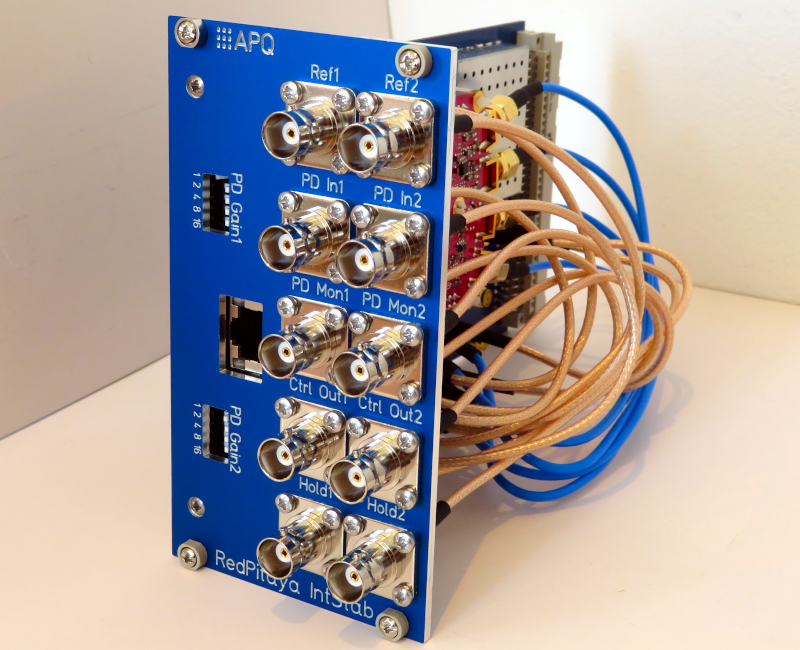
\includegraphics[width=\textwidth]{fig/intstab.png}
\end{maxipage}
\begin{abstract}
	The \href{https://github.com/TU-Darmstadt-APQ/RedPitaya-IntStab}{RedPitaya IntStab} is a fast digital controller for laser intensity stabilization featuring two independent channels. The commercial FPGA based \href{https://www.redpitaya.com/f130/STEMlab-board}{RedPitaya STEMlab 125-14} board is complemented by an analog interface that provides all necessary functionalities -- such as an input stage producing an error signal from a reference signal and a photodiode signal, a buffered control output and additonal monitoring outputs. The device is operated with the open-source software package \href{https://pyrpl.readthedocs.io/en/latest/}{PyRPL}.  
\end{abstract}
\tableofcontents

%%%%%%%%%%%%%%%%%%%%%%%%%%%%%%%%%%%%%%%%%%%%%%%%%%%%%%%%%%%%%%%%%%%%

\section{Setting up the RedPitaya}

\subsection{Mounting the RedPitaya on the IntStab PCB}

\index{RedPitaya OS}\marginlabel{Install the RedPitaya OS} Install the RedPitaya OS on a microSD card (4 GB min.) following the instructions on \href{https://redpitaya.readthedocs.io/en/latest/quickStart/SDcard/SDcard.html}{https://redpitaya.readthedocs.io/en/latest/quickStart/ SDcard/SDcard.html}. PyRPL has been tested with software release 0.94 to 0.99 as well as 1.04.  The latest release (2.05-37) does not work with our PyRPL branch so that using release 1.04-9 is recommended.  A local copy of this image can be found on $\backslash$$\backslash$brain43$\backslash$public$\backslash$Labortechnik $\backslash$Elektronik$\backslash$RedPitay$\backslash$Images. Older releases can be found on this website: \href{http://downloads.redpitaya.com/downloads/}{http://downloads.redpitaya.com/ downloads/}. Insert the card in the SD slot of the RedPitaya after installation.

\index{Offset resistors}\marginlabel{Remove the DC-offsets}
Remove the noisy DC-offset for both fast RedPitaya outputs by removing the four resistors marked in Fig.~\ref{fig:offset}. Use a standard soldering iron. This shifts the output voltage range from $\pm$\SI{1}{\volt} to \SI{0}{\volt}--\SI{2}{\volt}. Additional information can be found on \href{https://ln1985blog.wordpress.com/2016/02/07/red-pitaya-dac-performance/}{https://ln1985blog.wordpress.com/ 2016/02/07/red-pitaya-dac-performance/}. After removing the resistors, label the board accordingly (e.g. 'offset removed').

\textbf{Note:} The software (PyRPL and STEMlab) will still display and assume a $\pm$\SI{1}{\volt} range.

\textbf{Note:} The default output is now \SI{1}{\volt} instead of \SI{0}{\volt}.


\begin{figure}[H]
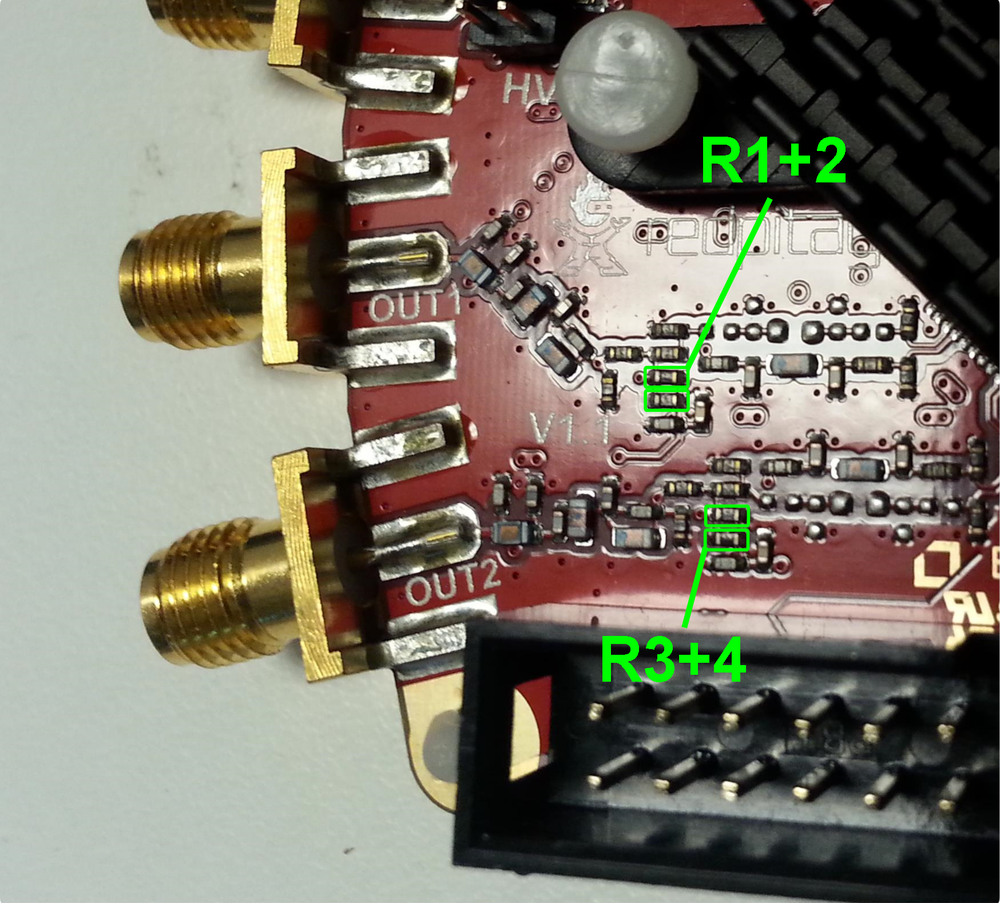
\includegraphics[width=\textwidth]{fig/offset-removal.png}
\caption{RedPitaya fast output offset resistors. [Image by L. Neuhaus]\label{fig:offset}}
\end{figure}

\index{Mount the RedPitaya}\marginlabel{Mount the RedPitaya board on the PCB}
Move the four nylon PCB mounts of the RedPitaya to the other side of the board. Attach \SI{17}{\milli\meter} hexnut M3 distance bolts to the PCB mounts using headless M3-screws. Connect the RedPitaya board (upside down) to the two 26-pin IDC-connectors on the PCB. Fix the board using M3 pan head screws and M3 washers.

\textbf{Note:} The RedPitaya's MAC address is denoted on the network connector. Make sure to remember it since it will not be visible after mounting the board. 

\textbf{Note:} Make sure all inputs are set to the low voltage range ('LV'). See also \href{https://redpitaya.readthedocs.io/en/latest/developerGuide/125-14/fastIO.html#analog-inputs}{https://redpitaya.readthedocs.io/en/latest/developer Guide/125-14/fastIO.html\#analog-inputs}.
\begin{figure}[H]
	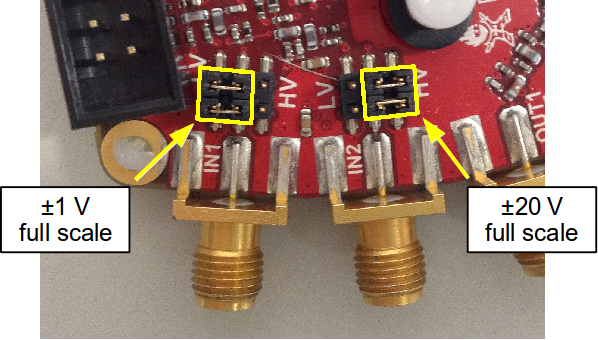
\includegraphics[width=\textwidth]{fig/Jumper_settings_photo.png}
	\caption{Jumper settings for $\pm$\SI{1}{\volt} and $\pm$\SI{20}{\volt} input range.\label{fig:jumper}}
\end{figure}
\begin{figure}[H]
	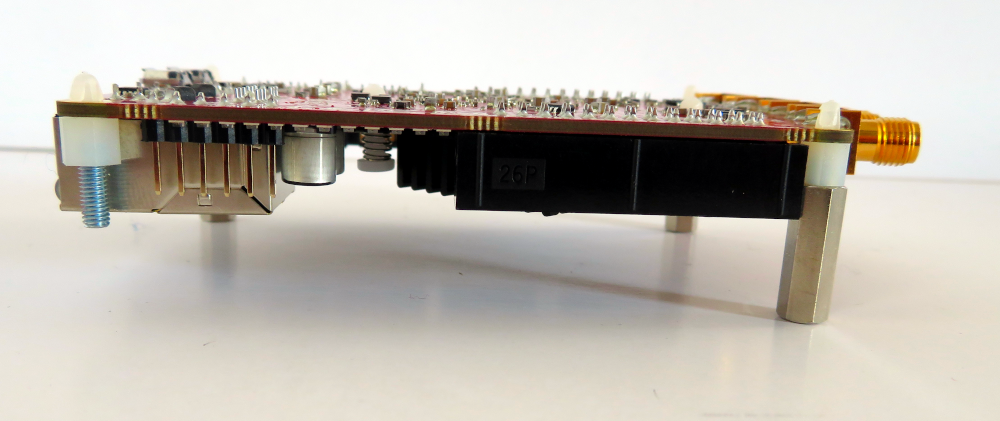
\includegraphics[width=\textwidth]{fig/mounting.png}
	\caption{RedPitaya board PCB mounting assembly.\label{fig:mounting}}
\end{figure}
\begin{figure}[H]
	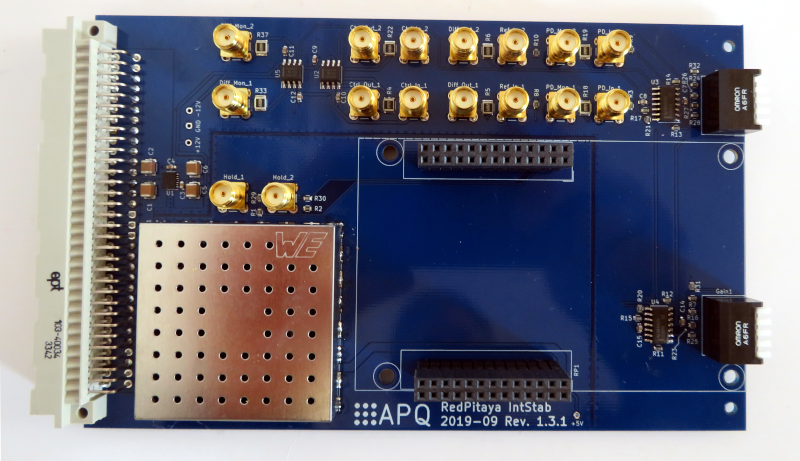
\includegraphics[width=\textwidth]{fig/PCB_intstab.png}
	\caption{Fully assembled RedPitaya IntStab PCB (Rev1.3.1).\label{fig:PCB}}
\end{figure}
\begin{figure}[H]
	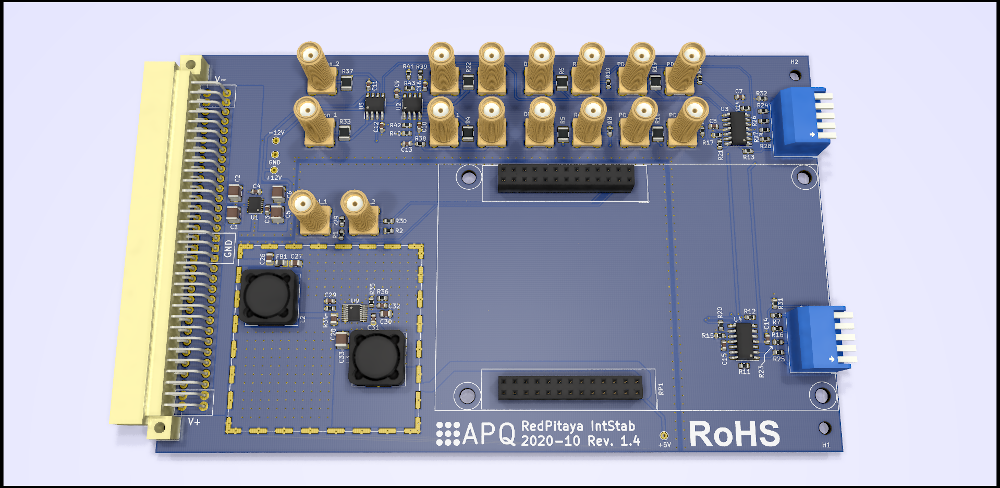
\includegraphics[width=\textwidth]{fig/RedPitaya_IntStab.png}
	\caption{3D-model of the latest PCB revision 1.4.\label{fig:PCB_3D}}
\end{figure}

\index{Front panel}\marginlabel{Install the frontpanel}
Use a pre assembled frontpanel and four additional \SI{20}{\centi\meter} SMA cables. Fix the frontpanel on the IntStab PCB using two \SI{10}{\milli\meter} pan head M2.5 screws and M2.5 washers. Connect the cable according the table below.

\begin{tabular}{|c|c|c|}\hline
\textbf{Front panel} & \textbf{PCB} 			& \textbf{RedPitaya}	\\\hline
Ref1		& Ref\_In\_1	& 	 		\\\hline	
PD In1		& PD\_In\_1		&			\\\hline
PD Mon1		& PD\_Mon\_1	&			\\\hline
Ctrl Out1	& Ctrl\_Out\_1	&			\\\hline
Hold1		& Hold\_1		& 			\\\hline
			& Ctrl\_In\_1	& Out1		\\\hline
			& Diff\_Out\_1	& In1		\\\hline
Ref2		& Ref\_In\_2	& 	 		\\\hline	
PD In2		& PD\_In\_2		&			\\\hline
PD Mon2		& PD\_Mon\_2	&			\\\hline
Ctrl Out2	& Ctrl\_Out\_2	&			\\\hline
Hold2		& Hold\_2		& 			\\\hline
 			& Ctrl\_In\_2	& Out2		\\\hline
 			& Diff\_Out\_2	& In2		\\\hline
\end{tabular}

\textbf{Note:} The \textit{Diff\_Mon} outputs on the PCB are optionally connected to an external frontpanel. Alternatively, they can be connected to the \textit{Hold} inputs on the frontpanel if the sample and hold feature is not used. In this case, label the frontpanel accordingly.

\begin{figure}[H]
	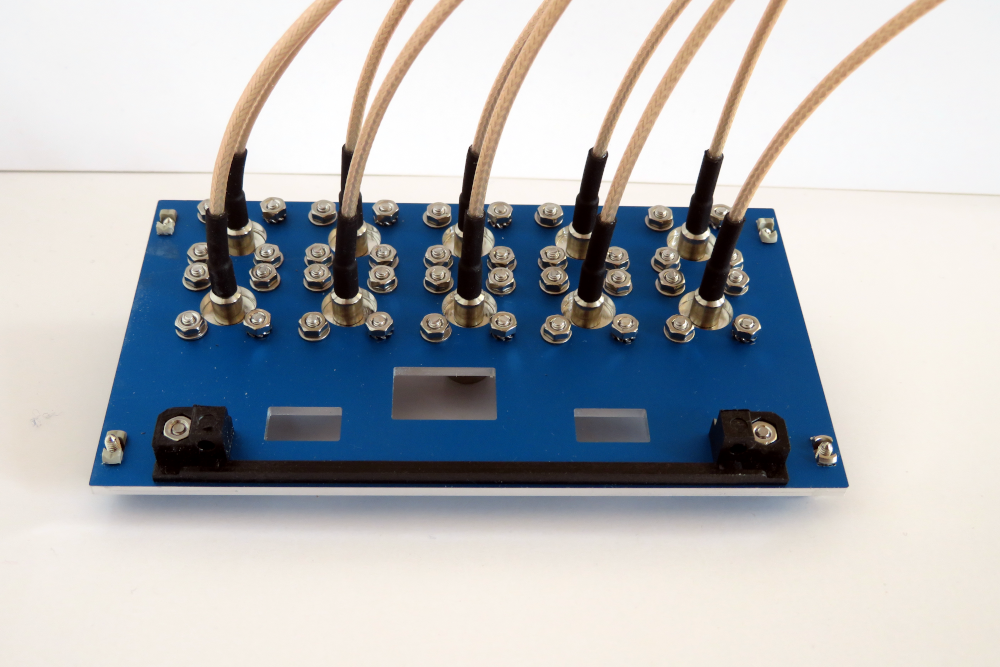
\includegraphics[width=\textwidth]{fig/front_panel.png}
	\caption{Pre-assembled frontpanel (RedPitaya IntStab).\label{fig:front_panel}}
\end{figure}

\subsection{Power supply and network connection}
\index{Power supply}\marginlabel{Power supply}
The RedPitaya lockbox is mounted in a 19-inch Fischer rack mount unit with our standard power supply (DIN41612 C64A/C connector). A $\pm$\SI{15}{\volt} supply is recommended. 

\begin{maxipage}
	\centering
	\begin{table}[H]
		{\small
		\begin{tabular}{|c|c|c|c|}\hline
			\textbf{Supply} & \textbf{Voltage range} & \textbf{Current@15\,V (typ./max.)}	& \textbf{Pin config. (default / Toptica)}  \\\hline
			V+			& 12.5\,V to 20\,V		& 	 0.35\,A / 1.00\,A					& 1A, 1C, 2A, 2C	/  31A, 31C	 \\\hline	
			V-			& -20\,V to -12.5\,V 	&		0.05\,A / 0.15\,A					& 31A, 31C, 32A 32C	/ 30A, 30C\\\hline	 
			GND			& -					&	-										& 16A, 16C, 17A, 17C, 18A, 18C  /  1A, 1C              \\\hline
		\end{tabular}
	}
		\caption{RedPitaya lockbox power supply rating. For connector pin configuration, see \href{https://b2b.harting.com/files/download/PRD/PDF_TS/0903164X921_100072506DRW176A.pdf}{Harting 09031646921}. \label{tab:power}}
	\end{table}
\end{maxipage}

\textbf{Note:} Always check the power supply polarity and current rating before connecting the controller. Permanent damage to the device may occur by reverse polarity. The RedPitaya requires a larger current while powering up.

\index{Network connection}\marginlabel{Network connection:} Connect the RedPitaya to the local network. The color code for RedPitaya network cables is blue. Per default the RedPitaya IP address is acquired via DHCP (see also next section). 

\section{Setting up the software}

\index{PyRPL}\marginlabel{Install PyRPL} 
The RedPitaya is operated with the Python software package PyRPL. You need a proper Python installation in order to run the software. For Windows OS, use \href{https://www.anaconda.com/}{Anaconda Python}. Create a virtual environment for PyRPL. Get \textit{pyrpl-env.yaml} from \href{https://github.com/TU-Darmstadt-APQ/RedPitaya-IntStab/tree/master/pyrpl}{https://github.com/TU-Darmstadt-APQ/RedPitaya-IntStab/tree/ master/pyrpl} and run (in the directory of the file)

\begin{tcolorbox}
	\begin{verbatim}
		conda env create -f pyrpl-env.yaml
	\end{verbatim}
\end{tcolorbox}

\textbf{Note:}  PyRPL is not compatible with the latest python and numpy version.

Activate the environment via

\begin{tcolorbox}
	\begin{verbatim}
		conda activate pyrpl-env
	\end{verbatim}
\end{tcolorbox}

Clone or download the branch 'external\_pid\_pause' from \href{https://github.com/lneuhaus/pyrpl/tree/external_pid_pause}{https://github.com/ lneuhaus/pyrpl/tree/external\_pid\_pause}. In the directory of the source files, run:

\begin{tcolorbox}
	\begin{verbatim}
		python setup.py develop
	\end{verbatim}
\end{tcolorbox}

\textbf{Note:} The branch 'external\_pid\_pause' is not the latest stable version of PyRPL. It will not be updated. If the installation does not work correctly and the sample and hold feature is not used, try installing the 'master' branch in a new environment.

\textbf{Known issues:}
\begin{itemize}
	\item 'pid'-module: Output limits seem to have a \SI{-1}{\volt} offset resulting in a max. output of \SI{0}{\volt}. Applying a \SI{1}{\volt} DC-offset with the 'asg'-module fixes the problem.
	\item 'lockbox' module: 'sweep' is only activated when the 'pid'-module is active.
\end{itemize}   

\index{IP and network}\marginlabel{Check the network connection and find the IP:}
The STEMlab web interface can be used for that task. Open this URL with a computer in the RedPitaya's local network:
\begin{tcolorbox}
	\begin{verbatim}
		http://rp-******.local
	\end{verbatim}
\end{tcolorbox}
Replace ****** by the last six digits of the RedPitaya's MAC address. Navigate to Settings$\rightarrow$Network in order to find the IP.

\textbf{Note:}
Label the frontpanel with the device IP, MAC-address and PCB revision.


\index{password}\marginlabel{Set the RedPitaya password} The default login for SSH connection to the RedPitaya is

\begin{tcolorbox}
	\begin{verbatim}
		User: root    Password: root
	\end{verbatim}
\end{tcolorbox}

Connect to the RedPitaya using a SSH terminal (e.g. \href{https://www.putty.org/}{putty}). The password can be changed with the command:
\begin{tcolorbox}
	\begin{verbatim}
		passwd
	\end{verbatim}
\end{tcolorbox}

\textbf{Note: }The password will be saved in plain text in the PyRPL config.-file. Do not reuse another password.

\index{Configure PyRPL}\marginlabel{Configure PyRPL}
Get the PyRPL example configuration file \textit{example\_intstab.yml} from \href{https://github.com/TU-Darmstadt-APQ/RedPitaya-IntStab/tree/master/pyrpl}{https://github.com/TU-Darmstadt-APQ/RedPitaya-IntStab/tree/ master/pyrpl}. Copy \textit{example\_intstab.yml} to \textit{$\backslash$pyrpl\_user\_dir$\backslash$config}. Rename the configuration file according to your application, open it with a text editor, and set the RedPitaya's IP (redpitaya>hostname:), password  (redpitaya>password:) and name of the application (pyrpl>name:). The default location of the \textit{pyrpl\_user\_dir} is \textit{C:$\backslash$Users$\backslash$USER}.

\index{Run PyRPL}\marginlabel{Run PyRPL}
After configuration, PyRPL can be started by activating the virtual environment and loading the configuration file (in a python terminal):

\begin{tcolorbox}
	\begin{verbatim}
		activate pyrpl-env
		python -m pyrpl your_config_file.yml
	\end{verbatim}
\end{tcolorbox}

For Windows OS, it is also possible to put the commands in batch-file after adding Anaconda to your path variable:

\begin{tcolorbox}
	\begin{verbatim}
		set PATH=%PATH%; C:\Users\USER\Anaconda3\Scripts
	\end{verbatim}
\end{tcolorbox}

Make sure the path to the Anaconda directory is correct. At the first start, open the 'lockbox' and 'scope' module and place the tabs at the right position. The changes are saved automatically to your configuration file.

\section{Connecting the RedPitaya IntStab to the experiment}

\subsection{Description of input and output functionalities}
The RedPitaya IntStab features two identical channels. All connections are labeled '1' and '2' accordingly. 

\index{PD In}\marginlabel{PD In}
High-Z input for the photodiode signal. The signal can be amplified internally. Input voltage range:  $\pm$\SI{10}{\volt}. Gain bandwidth product: \SI{35}{\mega\hertz}.


\index{Gain DIP switches}\marginlabel{Gain DIP switches}
Sets the photodiode gain between discrete values. Push the switch towards the number labels to close it. Open all other switches to set the denoted gain. It is also possible to combine the switches. The resulting gain $k$ from the set gains $k_1, k_2, \dots, k_n$ is


	$$k = 1+ \left(\sum_i(k_i -1)^{-1}\right)^{-1}$$
	
Note, that a larger gain will limit the bandwidth of the input stage. However, the bandwidth will be larger than the maximal control bandwidth of \SI{1.25}{\mega\hertz} for all applicable gains. 



\index{Ref In}\marginlabel{Err Mon}
High-Z input for the reference signal. The signal is buffered and subtracted from the amplified photodiode signal. The resulting error signal ('Diff\_Out') is fed to the RedPitaya input. Input voltage range:  $\pm$\SI{10}{\volt}. The RedPitaya input will saturate at $\pm$\SI{1}{\volt}. The rated max. input voltage for the RedPitaya is \SI{30}{\volt}. Gain bandwidth product: \SI{35}{\mega\hertz}. Note, that the subtracting amplifier stage has gain 2.

\index{Ctrl Out}\marginlabel{Ctrl Out}
Buffered and low-pass filtered output of the RedPitaya. Connect this output to the actuator, e.g. the intermediate port of a frequency mixer. The buffer can drive a \SI{50}{\ohm}-load at the maximal output voltage. Series resistance: \SI{50}{\ohm}.  Voltage range: 0--\SI{2}{\volt}. The default output voltage is \SI{1}{\volt} (due to the removed RedPitaya offsets).  Max. current: \SI{30}{\milli\ampere}. Cut-off frequency: \SI{5}{\mega\hertz}. The cut-off frequency can be altered by hardware modifications (see \href{https://github.com/TU-Darmstadt-APQ/RedPitaya-IntStab/tree/master/pcb}{schematics} for details).

\index{PD Mon}\marginlabel{PD Mon}
Monitoring output for the amplified photodiode voltage. Output voltage range: $\pm$\SI{10}{\volt}. Max. current: \SI{30}{\milli\ampere}. Series resistance: \SI{50}{\ohm}. Do not load the output with $Z < \SI{500}{\ohm}$.

\index{Hold}\marginlabel{Hold}
TTL-level logical input. If this input is pulled high, the P- and I-gains of the controller are set to zero with a \SI{150}{\nano\second} delay resulting in a constant control voltage. In this way a sample and hold feature is implemented. Input resistance: \SI{3}{\kilo\ohm}.

\index{Diff Mon} \marginlabel{Diff Mon}
Monitoring output for the error signal fed to the RedPitaya. Output voltage range: $\pm$\SI{10}{\volt}. Max. current: \SI{30}{\milli\ampere}. Series resistance: \SI{50}{\ohm}. Do not load the output with $Z < \SI{500}{\ohm}$. This output is not connected to the frontpanel per default.



\subsection{Hardware application notes \label{sec:app_note}}



\index{Control signal} \marginlabel{Control signal}
For our typical application, the control signal is applied to a diode-ring frequency mixer (e.g. MiniCircuits ZAD-3+) used as a variable RF-attenuator in order to control the RF-signal level of an AOM. Make sure the maximum ratings of the RF signal chain and the AOM are not exceeded when applying the full scale voltage to the intermediate port of the mixer. In order to minimize the influence of DAC quantization noise, it is also preferable to use the full output range for stabilization (i.e. the maximal intensity requires an RedPitaya output of approximately \SI{2}{\volt} ). This can be achieved by sufficient attenuation (usually \SIrange{6}{10}{\decibel}) of the RedPitaya's output.

\begin{figure}[H]
	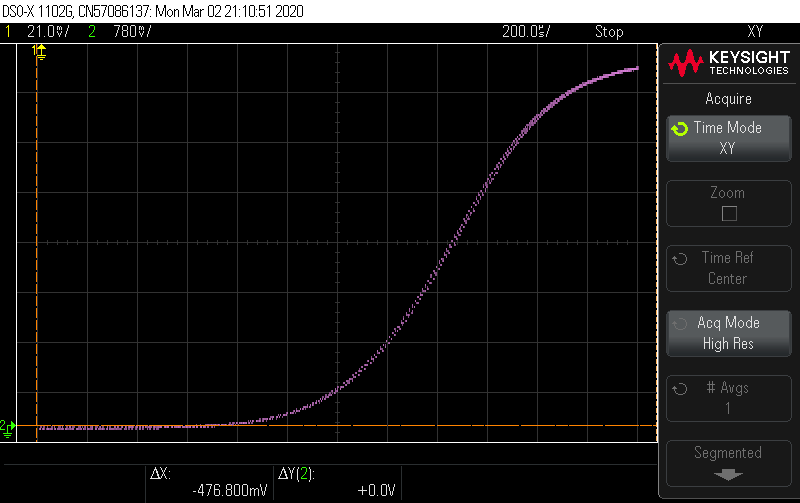
\includegraphics[width=\textwidth]{fig/mixer.png}
	\caption{Non-linear frequency mixer transfer function (Mini Circuits ZAD-3+). x (channel 1): Voltage at the intermediate port. y (channel 2): Photodiode signal (deflected intensity).  \label{fig:ZAD3}}
\end{figure} 

\index{External loop gain} \marginlabel{External loop gain}
The external loop gain is given by the ratio between a change in input signal (i.e. photodiode signal) and the change in output signal (Crtl Out) causing it. It determines the transfer function of the PI controller. Hence, an altered external loop gain requires adapted PI parameters. Note, that the external loop gain is sensitive to multiple changes in the setup, e.g. changes in the optical power applied to the AOM, the peak diffraction efficiency, the maximal RF-power,  the fraction of light guided to the photodiode, and the gain of the photodetector (including the gain setting of the RedPitaya IntStab). The external loop gain also depends on the laser intensity setpoint in relation to the maximally deflected intensity due to the non-linear relation between RF-power output of the frequency mixer and control voltage applied to the mixer.

  

\index{Input noise} \marginlabel{Input noise}
Ideally, the obtained intensity noise is limited by photodiode shot noise. In this case, the performance is enhanced by using more light for the stabilization, i.e. on the photodiode. All noise contributions on the reference signal and the photodiode signal (e.g. \SI{50}{\hertz} ground loops) within the control bandwidth are added to the laser intensity noise. In particular, large gain photodiode amplifiers are sensitive instruments. Try minimizing the 'dark' photodiode noise by sufficient shielding. For the reference signal, low-pass filtering might help if fast level transitions are not required.

\index{Control bandwidth} \marginlabel{Control bandwidth}
The maximal digital control bandwidth of the RedPitaya is \SI{1.25}{\mega\hertz} limited by a \SI{200}{\nano\second} propagation delay. The available bandwidth is determined by the phase margin given by the sum of all delays in the system. The phase margin is not necessarily linked to the amplitude transfer function. Several components in the system may induce delays: The AOM has a major share on the overall delay depending on the beam position in the crystal.\footnote{A typical speed of sound is \SI{4200}{\meter\per\second} resulting in a delay of \SI{240}{\nano\second} for a distance of \SI{1}{\milli\meter} between the active area and the RF actuator.} Also long cables or optical fibers may be relevant. Use a photodetetcor with a bandwidth well above \SI{1.25}{\mega\hertz}. Since the bandwidth of the RedPitaya's fast output is much larger than the control bandwidth, an additional output filter adapted to effective bandwidth of the system reduces the noise induced by the RedPitaya. 

\index{Saturation of the integrator}\marginlabel{Saturation of the integrator}
The digital integrator value has a saturation limit of 4 while the maximal output voltage corresponds to 1. Hence, if the control loop is closed, saturation of the output (e.g. if the setpoint cannot be reached) will only cause an additional delay comparable to the usual delay for transition to a different intensity level. This delay can be ignored if a minimal transition time is not required. In some cases, the control loop is not closed during the experiment. This is the case if the photodiode is blocked by a shutter or if a fast switch is used to control the RF power. In these cases, positive saturation (i.e. a I-value of +4) will lead to significant overshoot when closing the control loop. This can be avoided by setting appropriate reference levels while the control loop is not closed leading to a negative saturation of the output (i.e. a I-value of -4). Note, that most photodetectors have a significant negative offset requiring a negative setpoint. Alternatively, the sample and hold feature can be used.
 

\section{Intensity stabilization with PyRPL}

\subsection{PyRPL configuration}
The pre configured example uses the 'pid' module to implement two independent PI controllers and the 'scope' module to observe the error signal (Diff\_out).




\subsection{PyRPL settings}

\index{Input filters}\marginlabel{Input filters}
PyRPL allows to set four digital filters as input filters for the PI. Use this feature if the bandwidth of the photodetector is much larger than the control bandwidth.

\index{Sample and hold}\marginlabel{Sample and hold}
In the 'pid' module, set 'pause\_gains' to 'pi' if the sample and hold feature is used. The sample and hold feature can be activated manually by activating the 'paused' checkbox. Note, that the features are only available if the branch 'external\_pid\_pause' is installed.

\begin{figure}[H]
	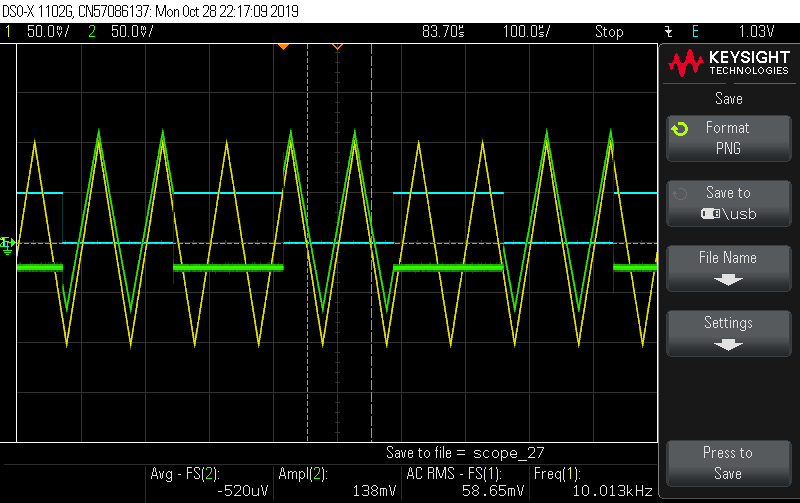
\includegraphics[width=\textwidth]{fig/sample_and_hold_P.png}\\
	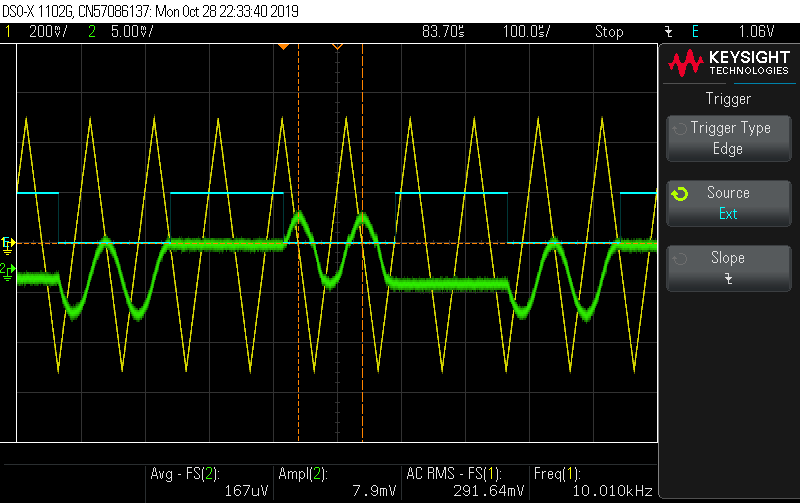
\includegraphics[width=\textwidth]{fig/sample_and_hold_I.png}
	\caption{Illustration of the sample and hold feature without feedback for a P-controller (top) and an I-controller (bottom). Blue: 'Hold' input. Yellow: RedPitaya input. Green: RedPitaya output. \label{fig:sample_and_hold}}
\end{figure}


\subsection{Set the PI parameters}

\index{Calibrate the ADC offset}\marginlabel{Calibrate the ADC offset}
The RedPitaya ADCs have considerable offsets and gain errors. The STEMlab software features a software calibration that is not used with PyRPL. Gain errors can be neglected since our setpoint is \SI{0}{\volt}. Nevertheless, the remaining offset leads to intensity offsets. The offsets have proven to be constant over time. In order to calibrate the input, terminate 'Ref' and 'PD In' with a \SI{50}{\ohm}-resistor (or short). Use the 'scope' module to determine the ADC DC-offset and set the 'setpoint' in the 'pid' module accordingly.


\index{Maximal photodiode voltage}\marginlabel{Maximal photodiode voltage}
Determine the maximal (amplified) photodiode level using the 'PD Mon' output. Deactivate the PI and set the respective output to '\SI{1}{\volt}' (i.e. \SI{2}{\volt}) using the 'asg' module. Increase the 'gain' using the DIP switches if the value is below \SI{1}{\volt}. If possible, increase the power at the photodiode instead of increasing the gain. 

\textbf{Note:}
If the external loop gain is changed the PI parameters must be adapted (see Section~\ref{sec:app_note} for details).

\index{I-gain}\marginlabel{I-gain}
Choose a setpoint of approximately \SI{50}{\percent} of the maximal photodiode voltage. Set the P-gain to zero and increase the I-gain until the system start to oscillate. Use half of this I-gain as a starting point.

\textbf{Note:}
In order to lock to a positive slope, the set PI-parameters in the 'pid' module have to be negative.

\index{Optimal PI parameters}\marginlabel{Optimal PI parameters}
Apply a short pulse (typically \SI{10}{\micro\second}) with a low repetition rate to the reference port and observe the 'PD Mon' output (and the reference pulse) using a scope with a signal generator. Choose the pulse height and offset such that both levels are in the linear region of the actuator (see Fig.~\ref{fig:ZAD3}). For the ZAD-3+, a transition from 25\% to 75\% of the maximal photodiode voltage is sufficient. Optimize the I-gain for minimal rise and fall times with minimal overshoot. Adding a small P-gain will allow for larger I-gains without oscillations/overshoot.

\textbf{Note:}
Due to the non-linearity of the mixer, the exact behavior of the controller depends on the setpoint in relation to the maximal photodiode level. E.g., a pulse from 0\% to 90\% will have larger rise and fall times or a pulse from 0\% to 50\% will be slightly asymmetric. The suggested optimization strategy yields a robust control performance avoiding oscillatory behavior and featuring decent transit times with minimal overshoot for all pulses. Additionally, these settings provide a maximal control bandwidth resulting in an optimal noise performance for a constant setpoint.

\textbf{Note:}
The exact performance (rise/fall times and delays) depends strongly on the AOM-type, the beam size, and position in the AOM since these parameters determine the available control bandwidth.          
\newpage

\begin{figure}[H]
	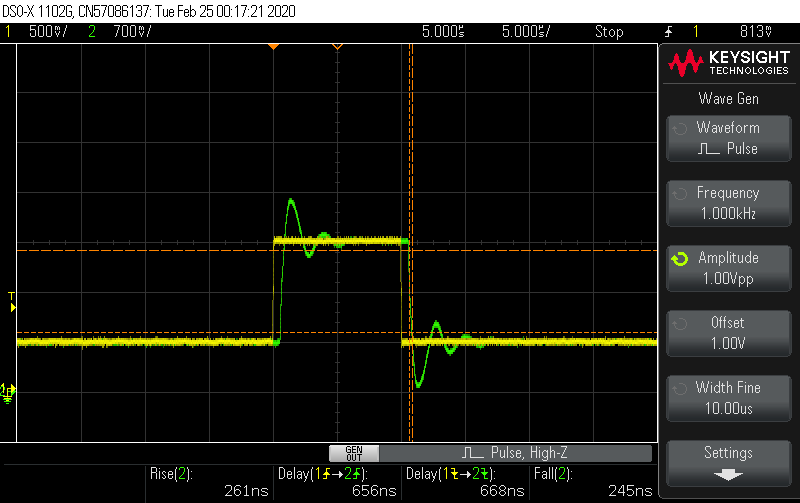
\includegraphics[width=\textwidth]{fig/I_high.png}\\
	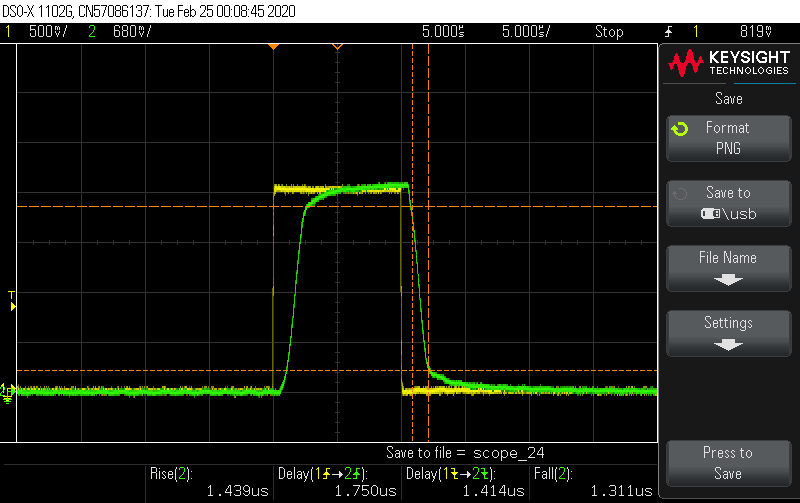
\includegraphics[width=\textwidth]{fig/I_low.png}\\
	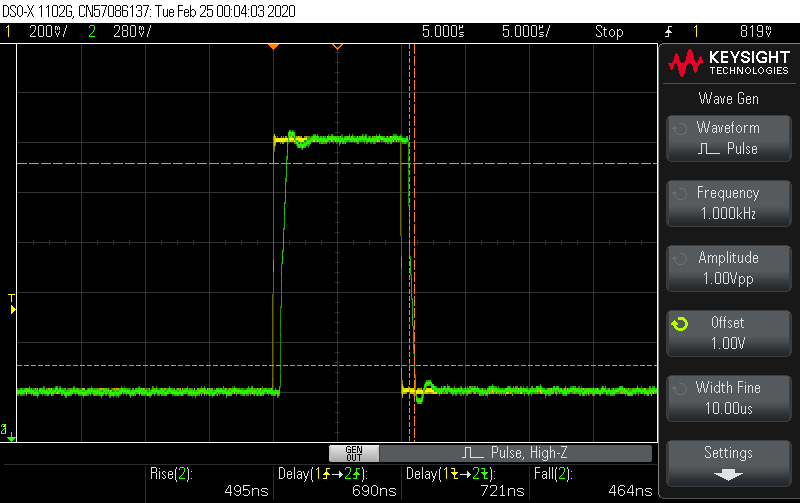
\includegraphics[width=\textwidth]{fig/I_opt.png}\\	
	\caption{Typical performance for different PI parameters. Top: I-gain too large. Centre: I-gain too small. Bottom: Optimal value.}
\end{figure}


\end{document}
